\subsection{Access from ordinary devices}\label{sec:eval:access}

The server never renders; every view is drawn by the client from the streamed octree. We replay the same scripted
60\,s camera flight over Shenzhen (5.0 million points, $1600\times900$ viewport, three repetitions) on three clients:
headless Chromium with an NVIDIA A100 on the server's local network, Chrome on an Apple M3 laptop streaming from the
server over the public internet, and Chromium with the SwiftShader software renderer, a stand-in for a device
without a usable GPU. The client reports its own frame intervals, the points it draws and the screen-space error it
achieves. We compare the adaptive budget (APH with CAS) against fixed point budgets of 100k, 1M (the Potree
default~\cite{schuetz2020octree}) and 3M points (Fig.~\ref{fig:stream}).

No fixed budget is right for every device. On both GPU clients every budget reaches the display rate (16.7\,ms per
frame), and the adaptive controller raises its budget to the top of its ladder: it draws as many points as the 3M
budget and reaches the same screen-space error, below one pixel (Fig.~\ref{fig:stream}b), whereas 100k points leave a
median error of 10--14\,px. On the software renderer the picture reverses. With 1M or 3M points it renders at 12\,fps,
with a median frame time of 67--83\,ms and 83--85\% of frames beyond 1.5 times its 33.3\,ms target. The adaptive
controller holds the target (95th-percentile frame time 33.3\,ms, no frame beyond 1.5 times the target) and still draws
1.5 times as many points as the 100k budget, with a lower error (6.7 against 9.2\,px). Point selection costs at most
0.4\,ms per frame (95th percentile) on every client; slowing the M3's CPU four-fold by emulation changes neither its
frame times nor its error. The first view appears 1--2\,s after opening the page on the local network and after 14\,s
over the internet, where the 1.5\,MB first screen and the 22\,MB streamed during the flight compete with the path's
bandwidth. Because the server only serves static byte ranges and all selection runs in the client, adding viewers
adds file traffic but no per-viewer computation on the server; we did not measure many concurrent viewers.

\begin{figure}[t]
\centering
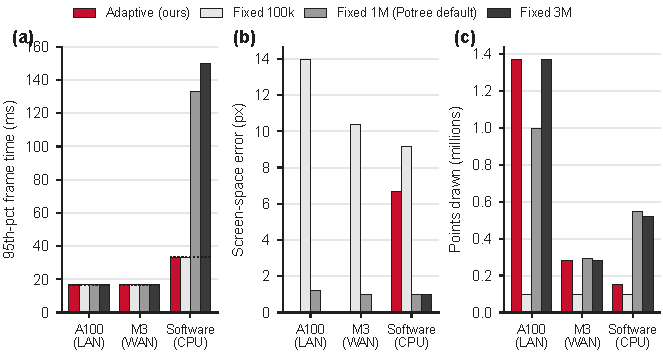
\includegraphics[width=\textwidth]{figures/pdf/stream.pdf}
\caption{The same 60\,s camera flight over Shenzhen on three clients, adaptive budget vs fixed budgets; medians of three
runs. (a) 95th-percentile frame time, with each client's frame target dotted. (b) Median screen-space error of the drawn
view. (c) Median number of points drawn}
\label{fig:stream}
\end{figure}
